\documentclass[aspectratio=169]{beamer}
\beamertemplatenavigationsymbolsempty
%\setbeameroption{show only notes}
%\setbeameroption{show notes on second screen}

\usepackage{pdfpages}
\usepackage{graphicx}
\graphicspath{{figures}{figures/graphics}}


\usepackage{tikz}
\usepackage{tikzscale}
\usetikzlibrary{shapes, arrows.meta, positioning, calc, intersections}
\tikzstyle{block} = [rectangle, draw, rounded corners]


\usepackage[export]{adjustbox}

\usepackage{caption}
\captionsetup[figure]{labelformat=empty, font=scriptsize, labelfont=scriptsize}

\usepackage{subcaption}
\usepackage{multicol}

\usepackage[super, sort&compress]{natbib}
\bibliographystyle{unsrtabbrv}

\usepackage[normalem]{ulem}

\definecolor{palatinatepurple}{rgb}{0.41, 0.16, 0.38}

\hypersetup{
	colorlinks=true,
	linkcolor=black,
	citecolor=black,
	urlcolor=palatinatepurple
}

% beamer style
\setbeamertemplate{blocks}[rounded][shadow]
\setbeamercolor{block body}{bg=structure!10}
\setbeamercolor{block title}{bg=structure!20}

\setbeamercolor{block body example}{bg=green!10}
\setbeamercolor{block title example}{bg=green!20}

\setbeamercolor{block body alerted}{bg=red!10}
\setbeamercolor{block title alerted}{bg=red!20, fg=black}



% just have frame number in footline
\setbeamertemplate{footline}[frame number]

\def\swidth{2cm}
\usetheme[width=\swidth]{Hannover}
%\usecolortheme{}

%%%%% ADD  NOPHOTO Icon

%
\makeatletter
\addtobeamertemplate{sidebar left}{}{%
	\begin{minipage}{\swidth}
		\centering
%		\includegraphics[width=0.3\textwidth]{../../../pres-images/no-photo}
		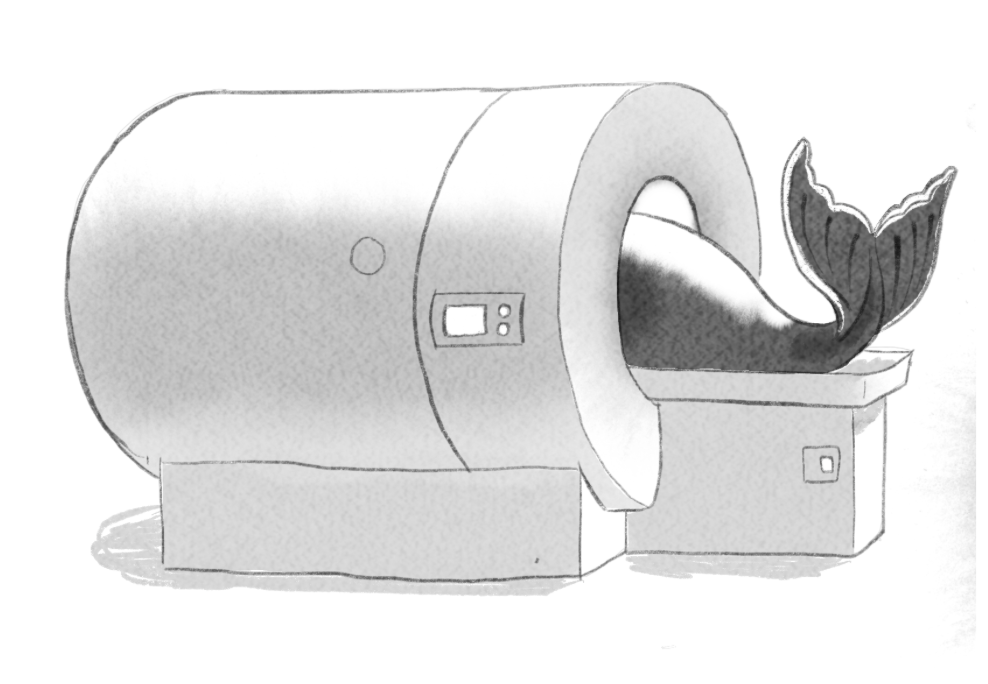
\includegraphics[width=1.5cm]{complexwhale}
		\vspace{2em}
	\end{minipage}
	
}
\makeatother

%%%%%

% numberless footnote
\newcommand\blfootnote[1]{%
	\begingroup
	\renewcommand\thefootnote{}\footnote{#1}%
	\addtocounter{footnote}{-1}%
	\endgroup
}



\title[Brainwise Wordsearch]{Lexical Methodological Exploration of Neuroimaging Studies}
\subtitle[]{PoCS2 Project Update}

%\date{}

\author[Tony Barrows]{Tony Barrows}

%\institute[UVM]{ 
\includegraphics[width=4cm]{larner}}

%\institute{\inst{1} University of Vermont \and \inst{2} University of Michigan}

\begin{document}
	
	\begin{frame}
		\maketitle
		
		\centering
%		\includegraphics[width=2cm]{../../../pres-images/20150925-ABCD}
		
\includegraphics[width=3cm]{larner}
		
\includegraphics[width=3cm]{nerve}
		
\includegraphics[width=2cm]{complexsystems}
		
\includegraphics[width=2cm]{complexbrain}
%		
\includegraphics[width=2cm]{../../../pres-images/complexsystems}
%		\includegraphics[width=3cm]{../../../pres-images/vacc_green}
	\end{frame}
	
	%% Outline
%\begin{frame}{Outline}
%	\tableofcontents
%\end{frame}

\section{Introduction}

\begin{frame}{Introduction}
	\textbf{Motivation:} Describe the state of the field in neuroimaging research
	\vspace{5mm}
	\begin{columns}
			\column{0.2\textwidth}
			\includegraphics[width=\columnwidth]{papers/Marek22}
			\column{0.8\textwidth}
			\href{https://www.nature.com/articles/s41586-022-04492-9}{Reproducible brain-wide association studies require thousands of individuals \cite{MarekEtAl2022}}
			
			Reasons:
			\begin{itemize}
					\item Fishing for statistical significance (``p-hacking'') \cite{Nuzzo}
					\item Overfitting \cite{Hawkins2004}
					\item Confirmation and publication biases \cite{Bishop2020}
					\item \textbf{Variability in methods \cite{Botvinik-NezerEtAl2020}} 
				\end{itemize}
		\end{columns}
	
	
\end{frame}


%\begin{frame}{(Very) High-level overview of Functional Magnetic Resonance Imaging (fMRI):}
%	\includegraphics[width=\linewidth]{mri_diagram}
%	\blfootnote{Images from NIMH and \cite{Siden2020}}
%\end{frame}







\section{Methods}

\begin{frame}{Dataset}
	
	\begin{columns}[t]
		\column{0.5\textwidth}
		
\includegraphics[width=0.5\textwidth]{neurosynth}\cite{YarkoniEtAl2011}
		
		\begin{itemize}
			\item 14,371 studies
			\item 1,334 terms
			\item Focuses on specific inference
		\end{itemize}
		
		\column{0.5\textwidth}
		
\includegraphics[width=0.5\textwidth]{neuroquery}\cite{DockesEtAl2020}
		
		\begin{itemize}
			\item 13,459 studies
			\item 7,547 terms
			\item Focuses on multivariate prediction (across related terms)
			\begin{itemize}
				\item e.g., you enter \texttt{calculation}, it also searches \texttt{computation}
			\end{itemize}
		\end{itemize}
	\end{columns}
	
	\begin{block}{}
		Each works by finding relationships between \textbf{terms} and \textbf{brain activation} by extracting standardized coordinates from results
	\end{block}
\end{frame}


\begin{frame}{Dataset}

	\begin{columns}[t]
		\column{0.5\textwidth}
			
\includegraphics[width=0.5\textwidth]{neurosynth}\cite{YarkoniEtAl2011}
			
			\begin{itemize}
				\item 14,371 studies
				\item 1,334 terms
				\item Focuses on specific inference
			\end{itemize}
			
		\column{0.5\textwidth}
			
\includegraphics[width=0.5\textwidth]{neuroquery}\cite{DockesEtAl2020}
			
			\begin{itemize}
				\item \sout{13,459 studies}
				\item \sout{7,547 terms}
				\item \sout{Focuses on multivariate prediction (across related terms)}
				\begin{itemize}
					\item \sout{e.g., you enter \texttt{calculation}, it also searches \texttt{computation}}
				\end{itemize}
			\end{itemize}
	\end{columns}
	
	\begin{block}{}
				Each works by finding relationships between \textbf{terms} and \textbf{brain activation} by extracting standardized coordinates from results
	\end{block}
\end{frame}



\begin{frame}{Automated text-to...methods?}
	\begin{itemize}
		\item Meta-analysis help overcome problems related to p-hacking, overfitting, and confirmation bias
		\begin{itemize}
			\item $\rightarrow$ but not \textbf{variability in methods}
		\end{itemize}

	\end{itemize}
	
	\vspace{3mm}
	
	\pause
	Proposal:
	
	\begin{itemize}
		\item Use text from \texttt{neurosynth} and \texttt{NeuroQuery} to describe the field:
		\begin{itemize}
			\item Common methods for each type of question
			\item Results patterns associated with different techniques
		\end{itemize}
	\end{itemize}
\end{frame}

\begin{frame}{Automated text-to...methods?}
	\begin{itemize}
		\item Meta-analysis help overcome problems related to p-hacking, overfitting, and confirmation bias
		\begin{itemize}
			\item $\rightarrow$ but not \textbf{variability in methods}
		\end{itemize}
		
	\end{itemize}
	
	\vspace{3mm}
	
	Proposal:
	
	\begin{itemize}
		\item Use text from \texttt{neurosynth} \sout{and \texttt{NeuroQuery}} to describe the field:
		\begin{itemize}
			\item \textbf{Common methods} \sout{for each type of question}
			\item \sout{Results patterns associated with different techniques}
		\end{itemize}
	\end{itemize}
\end{frame}

\begin{frame}{Methods}
	\begin{enumerate}
		\item Manually construct a corpus of methods-related words from a random sample of abstracts
		\item Implement a set-logic-based algorithm to
			\begin{enumerate}
				\item Slice off the beginnings and ends of abstracts
				\item Decide if what remains is ``methods''
			\end{enumerate}
		\item Use two popular topic modeling approaches (latent Dirichlet allocation (LDA)\cite{Blei2003} and \texttt{BERTopic}\cite{Grootendorst2022a}) to \sout{haul out} extract relevant topics
		\begin{itemize}
			\item Do this for all ($n=12,781$) abstracts, within several time-period subsets
		\end{itemize}
	\end{enumerate}
	
	\blfootnote{Thanks to Jay Lobell for the suggestion to use topic modeling}
\end{frame}

\section{Results}



\begin{frame}{Results -- First Topics}

	
	\includegraphics[width=\textwidth]{figures/project/top_n_topics_pres}
	
	\blfootnote{List of methods-related terms is available in the paper}
\end{frame}

\begin{frame}{Results -- Topics Over Time}
	
	\includegraphics[width=\textwidth]{figures/project/topics_by_timepoint}
\end{frame}

\section{Conclusion}

\begin{frame}{Conclusion}
	\begin{itemize}
		\item Implemented a method for exploring a sub-section of scientific texts
		\item Directly compared the utility of two popular topic modeling approaches in this context
		\item Laid groundwork for full-text analysis
	\end{itemize}
\end{frame}



%
%\begin{frame}{Things to do}
%		
\includegraphics[width=0.15\textwidth]{neuroquery}
%		appears to contribute 4,777 \textbf{unique} articles $\ldots$ but with no dates \footnote[1]{%
%		\tiny Hours spent writing elegant script to query APIs only to realize the metadata isn't available for a reason: 5+}
%		
%		\vspace{3mm}
%		
%		We'll stick with \texttt{neurosynth} for now.
%		
%		\begin{columns}
%			\column{0.75\textwidth}
%					\includegraphics[width=\columnwidth]{figures/project/ns_pubcount.pdf}
%					
%			\column{0.25\textwidth}
%				\begin{itemize}
%					\item Try to solve $\uparrow$
%					\item Generate methods words (buckets)
%					\item Drop papers into buckets
%					\item Look for developments over time
%				\end{itemize}
%		\end{columns}
%
%\end{frame}



\begin{frame}[allowframebreaks]{References}

		\tiny
		\bibliography{zotero}

\end{frame}


	
	
\end{document}

